In task 2 we want to generate a desired (smooth) state$-$input curve and perform the trajectory generation task of Task 1 on this new desired trajectory.

In order to generate a smooth state-input curve we opted for a sigmoid trajectory that starts on the first equilibrium state and finishes on the second one.
The sigmoid function, often denoted as $\sigma(x)$, is defined as:
\[
\sigma(x) = \frac{1}{1 + e^{-x}}
\]
The Figure below illustrates the behavior of the sigmoid function.

\begin{figure}[h]
  \centering
  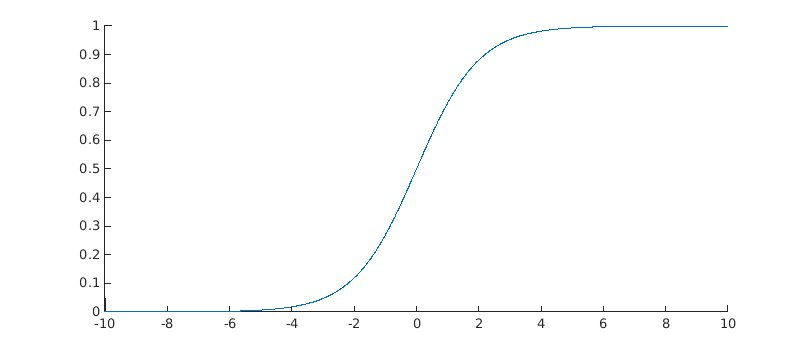
\includegraphics[width=0.6\textwidth]{pictures/sigmoide_graph.png}
  \caption{Behaviour of the sigmoid}
  \label{fig:sigmoid_plot}
\end{figure}

The choice of reference trajectory plays a crucial role in the performance and convergence characteristics of the Linear Quadratic Regulator (LQR) algorithm, it trapresents a more feasible reference for the trajectory.

The continuity of a smooth trajectory can facilitate the convergence of the LQR algorithm, as the system can gradually adapt to reference variations.

Furthermore, a smooth trajectory can help minimize the control energy required by the system. If the trajectory is already "close" to the optimal solution, the LQR algorithm may converge more quickly than in a situation where the reference has sharp changes.

\section{Results}
In this section, we present the outcomes of the Linear Quadratic Regulator on a sigmoid reference trajectory.

We applied this method to two different cases. In the first case, the equilibria are two distinct positions in space, and in the second case they are two distinct constant linear velocities. In the second case the trajectory for the state relative to the position x and y is obtained with the integration of the speed reference.

An example of the two cases follows:

\begin{figure}[H]
  \centering
  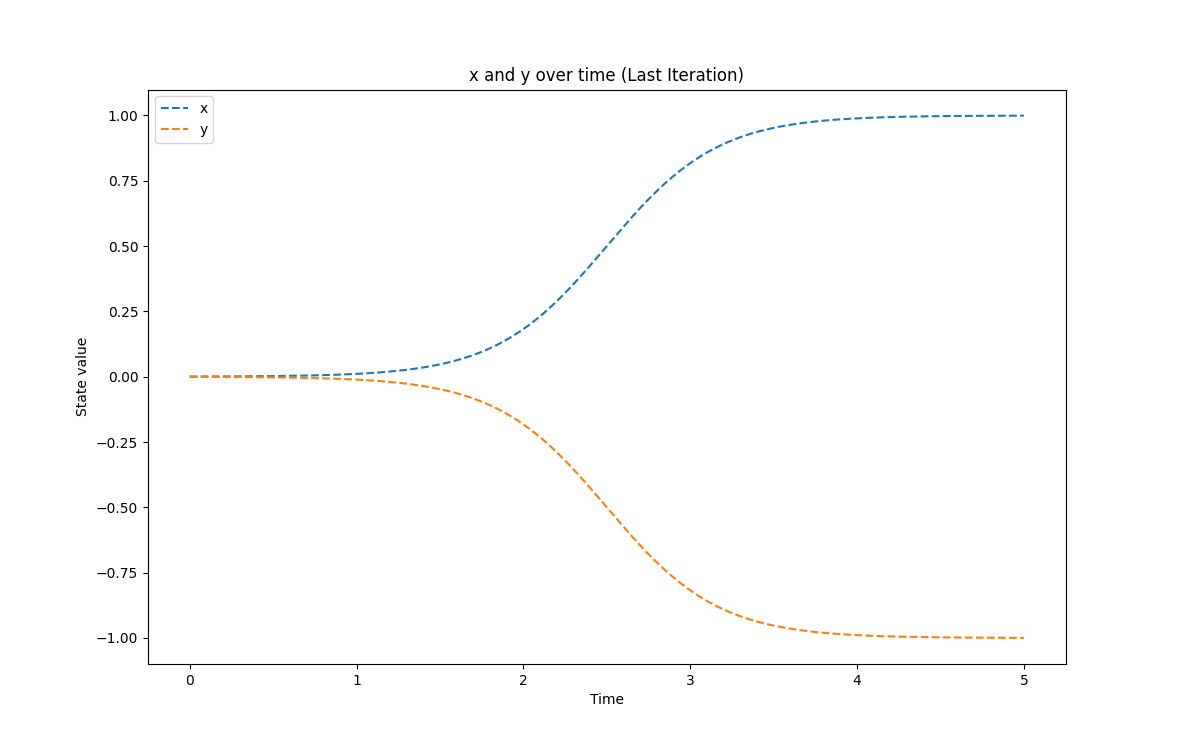
\includegraphics[width=0.6\textwidth]{pictures/Figure_1_posizione_smooth}\hfill
  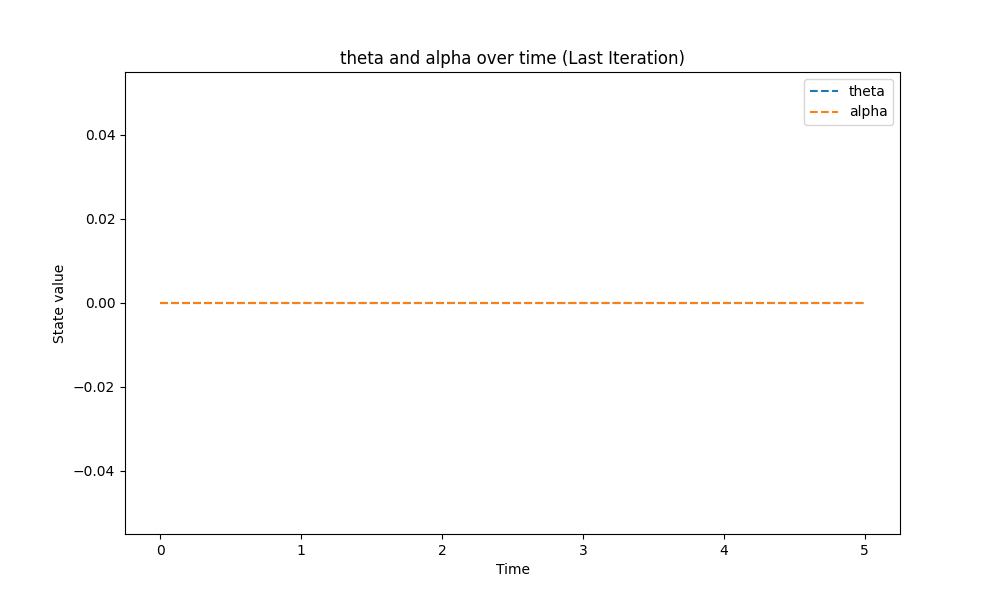
\includegraphics[width=0.6\textwidth]{pictures/Figure_2_posizione_smooth}\hfill
  \caption{Case 1: configuration reference over time.}
  \label{fig:Reference trajectory}
\end{figure}

\begin{figure}[H]
  \centering
  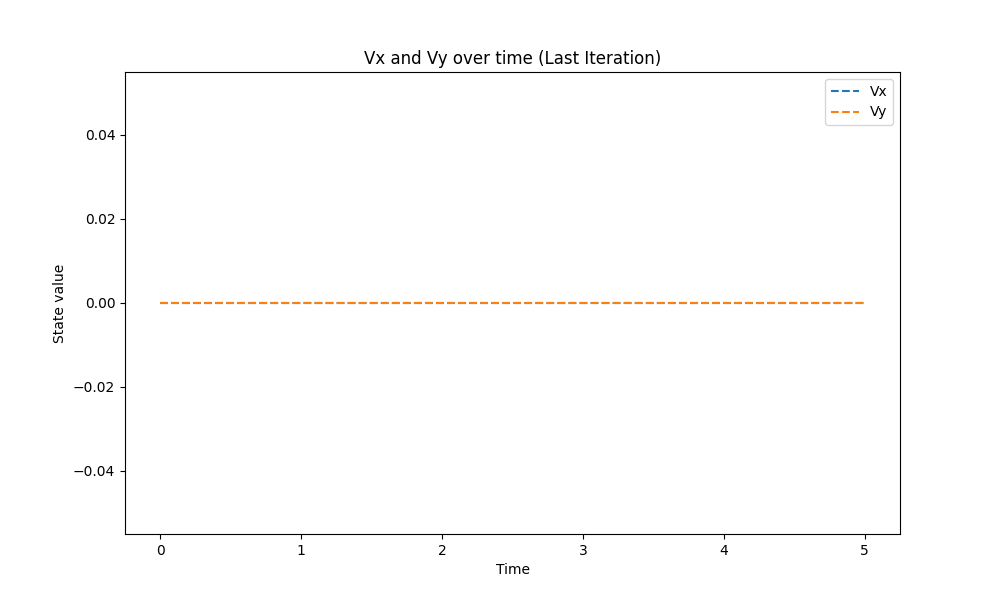
\includegraphics[width=0.85\textwidth]{pictures/Figure_3_posizione_smooth}\hfill \\
  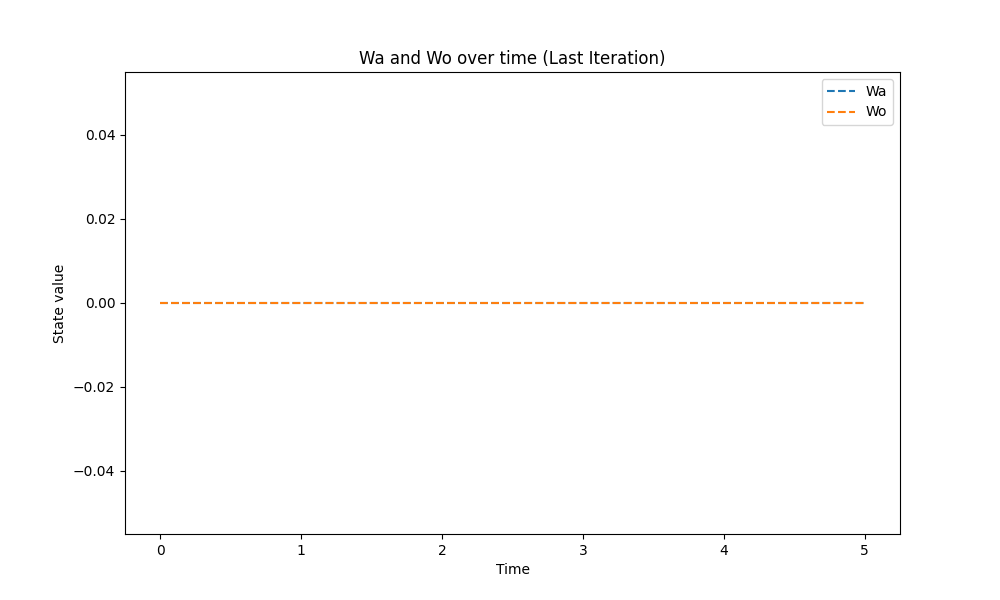
\includegraphics[width=0.85\textwidth]{pictures/Figure_4_posizione_smooth}\hfill
  \caption{Case 1: velocities reference over time.}
  \label{fig:Reference trajectory}
  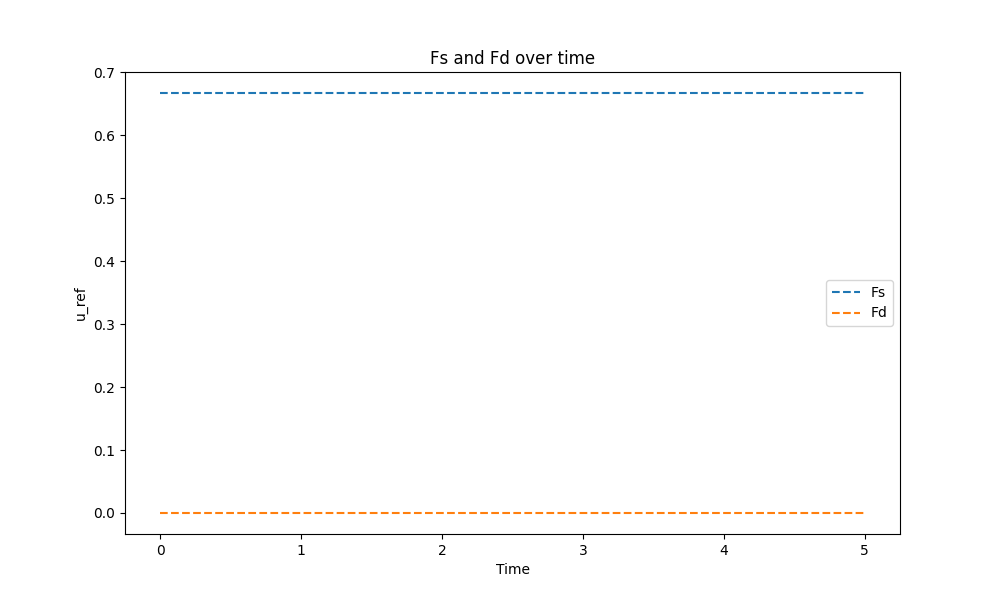
\includegraphics[width=0.85\textwidth]{pictures/Figure_5_posizione_smooth}
  \caption{Case 1: Input reference over time.}
  \label{fig:Reference trajectory}
\end{figure}

\begin{figure}[H]
  \centering
  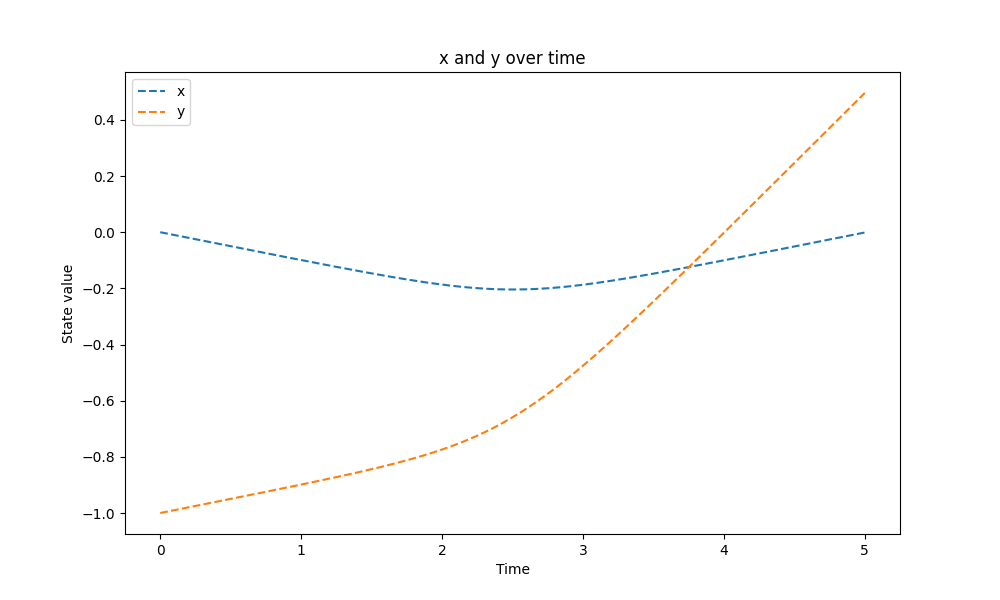
\includegraphics[width=0.9\textwidth]{pictures/Figure_1_velocita_smooth}\hfill\\
  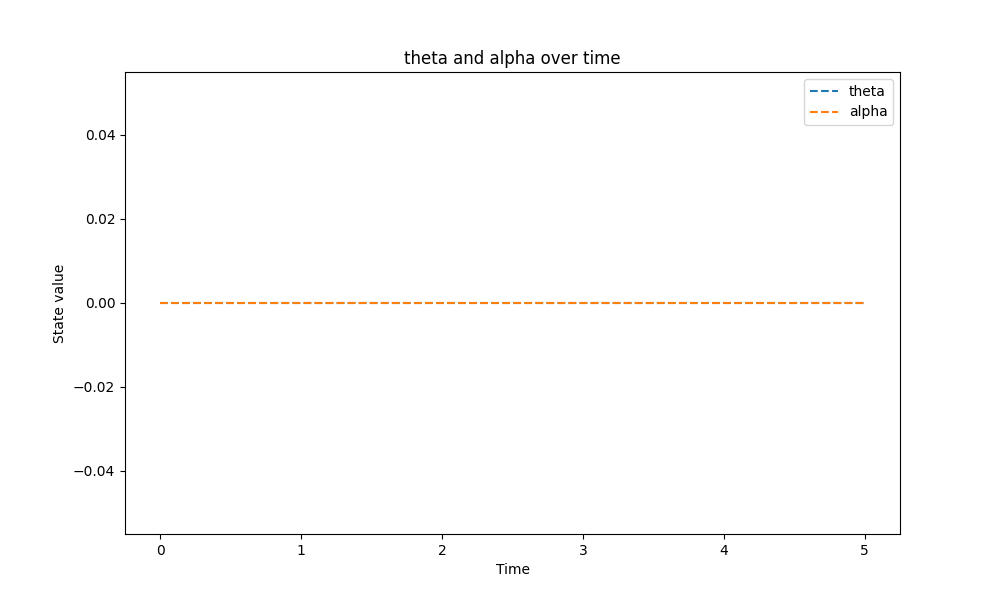
\includegraphics[width=0.9\textwidth]{pictures/Figure_2_velocita_smooth}\hfill
  \caption{Case 2: configuration reference over time.}
  \label{fig:Reference trajectory}
\end{figure}

\begin{figure}[H]
  \centering
  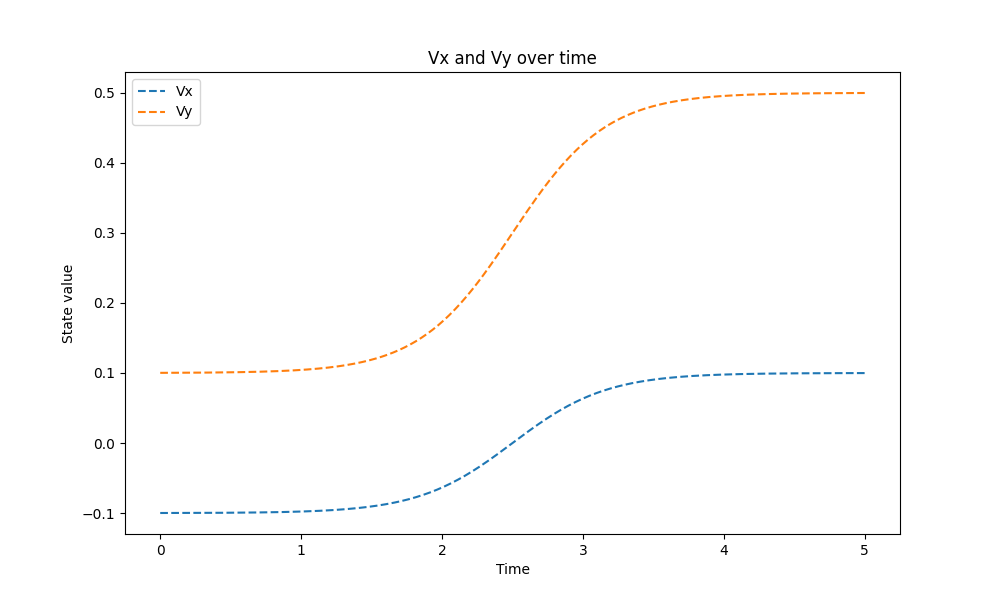
\includegraphics[width=0.85\textwidth]{pictures/Figure_3_velocita_smooth}\hfill \\
  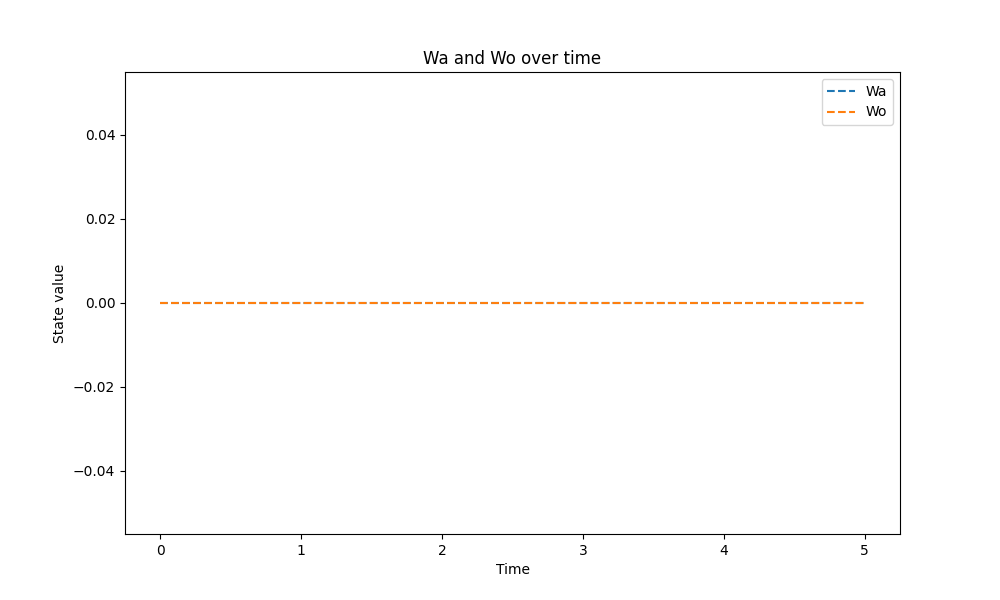
\includegraphics[width=0.85\textwidth]{pictures/Figure_4_velocita_smooth}\hfill
  \caption{Case 2: velocities reference over time.}
  \label{fig:Reference trajectory}
  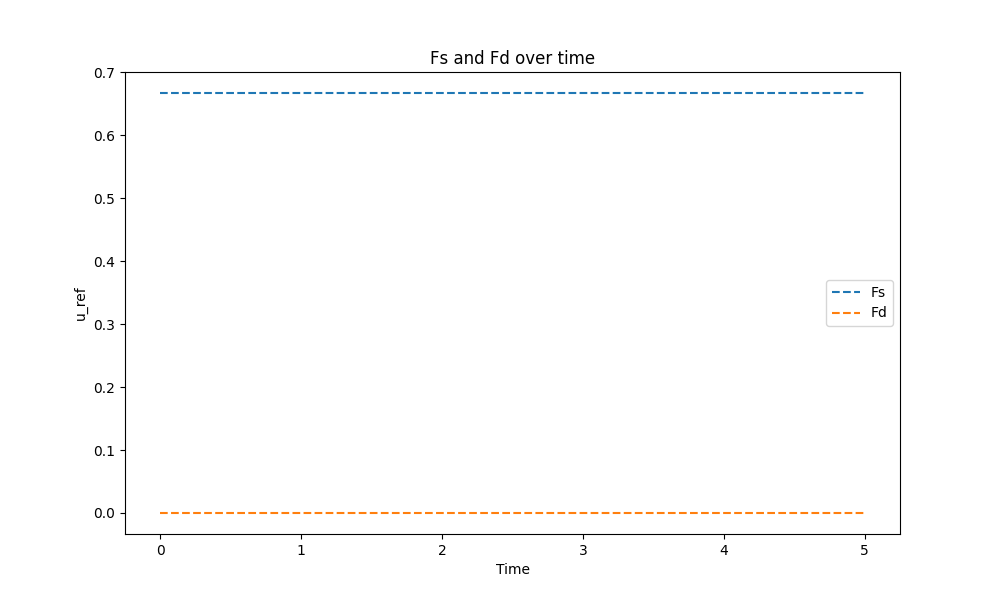
\includegraphics[width=0.85\textwidth]{pictures/Figure_5_velocita_smooth}
  \caption{Case 2: Input reference over time.}
  \label{fig:Reference trajectory}
\end{figure}

\subsection{Optimal trajectory}
In this section, we present the outcomes of the Linear Quadratic Regulator on the reference trajectory provided by equilibria that are two distinct positions in space (Case 1).

In the following pages the optimal trajectory found by our algorithm is shown.

\begin{figure}[H]
  \centering
  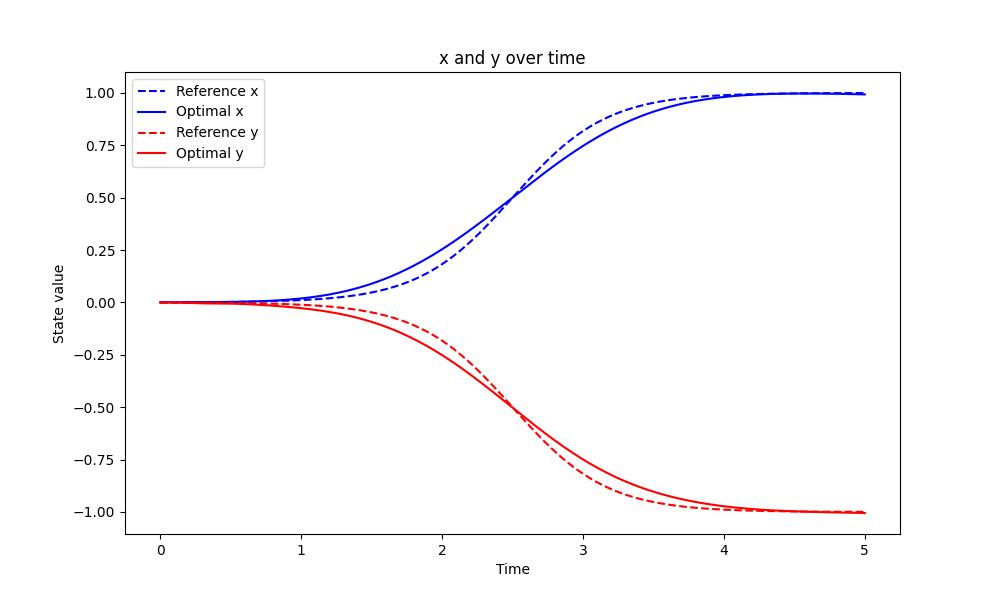
\includegraphics[width=0.9\textwidth]{pictures/Figure_1_opt_smooth.png}\hfill 
  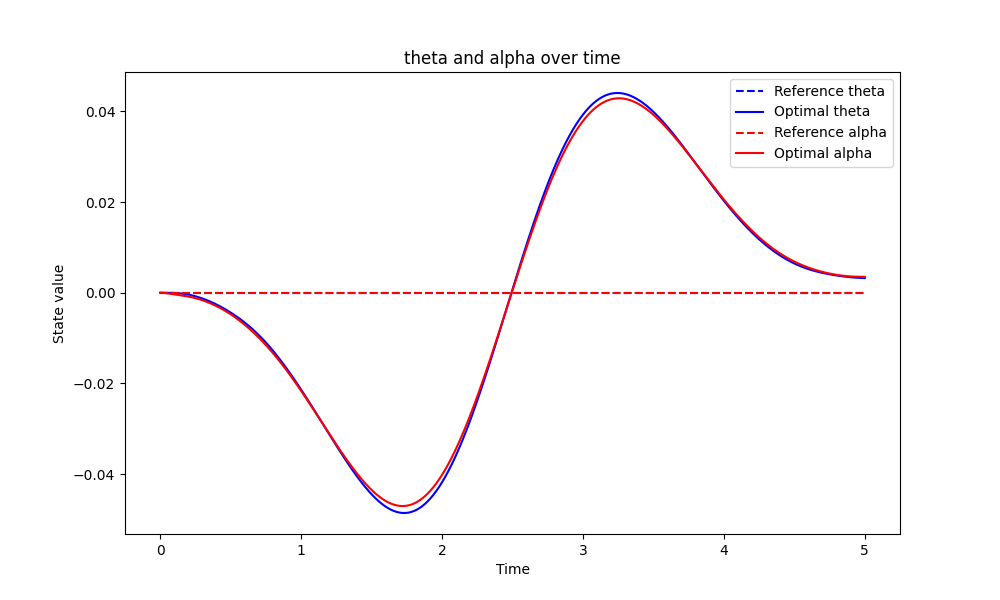
\includegraphics[width=0.9\textwidth]{pictures/Figure_2_opt_smooth.png}\hfill
  \caption{Optimal configuration over time.}
  \label{fig:Reference trajectory}
\end{figure}

\begin{figure}[H]
  \centering
  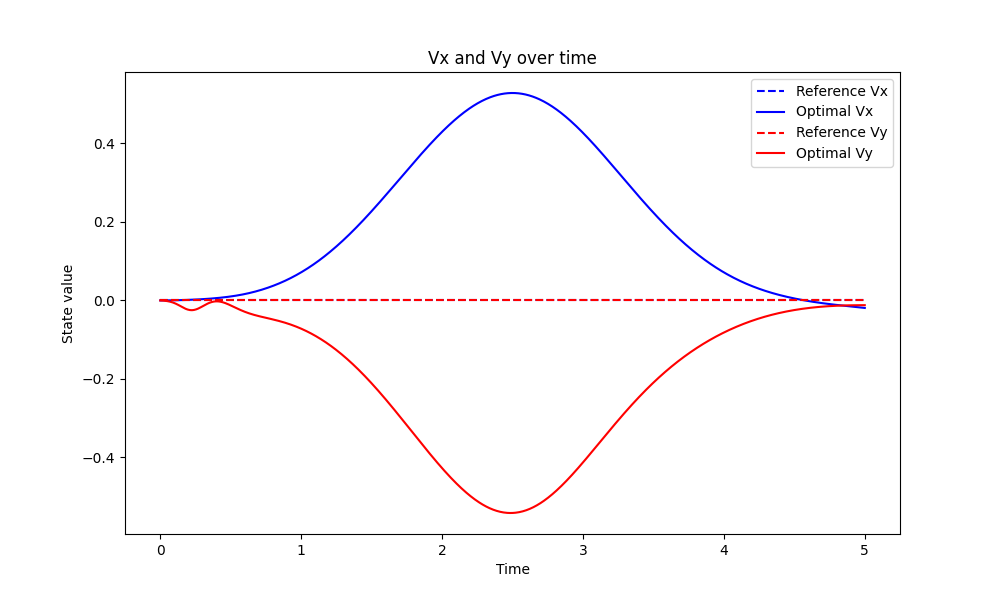
\includegraphics[width=0.85\textwidth]{pictures/Figure_3_opt_smooth.png}\hfill \\
  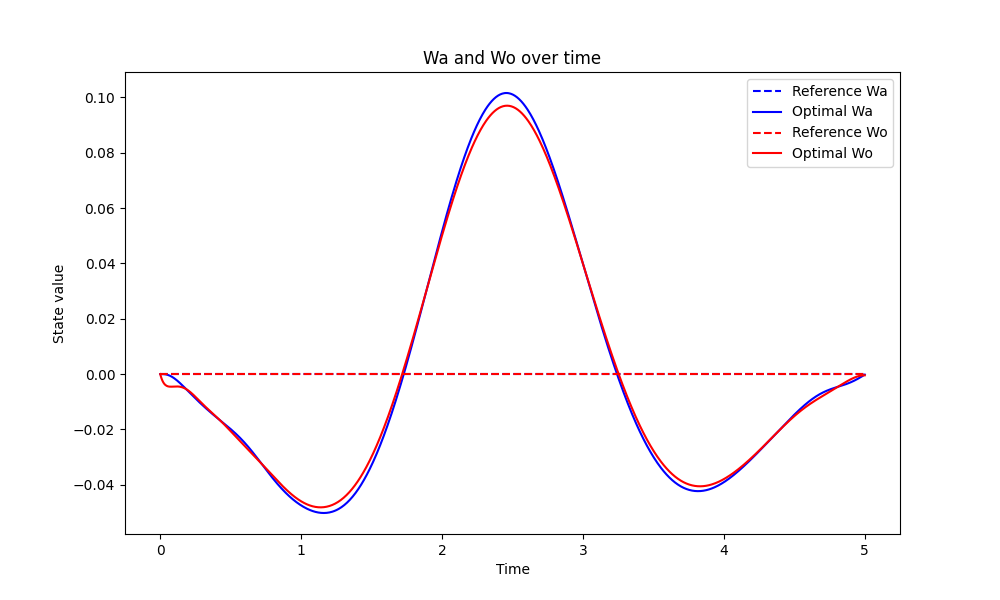
\includegraphics[width=0.85\textwidth]{pictures/Figure_4_opt_smooth.png}\hfill
  \caption{optimal velocities over time.}
  \label{fig:Reference trajectory}
  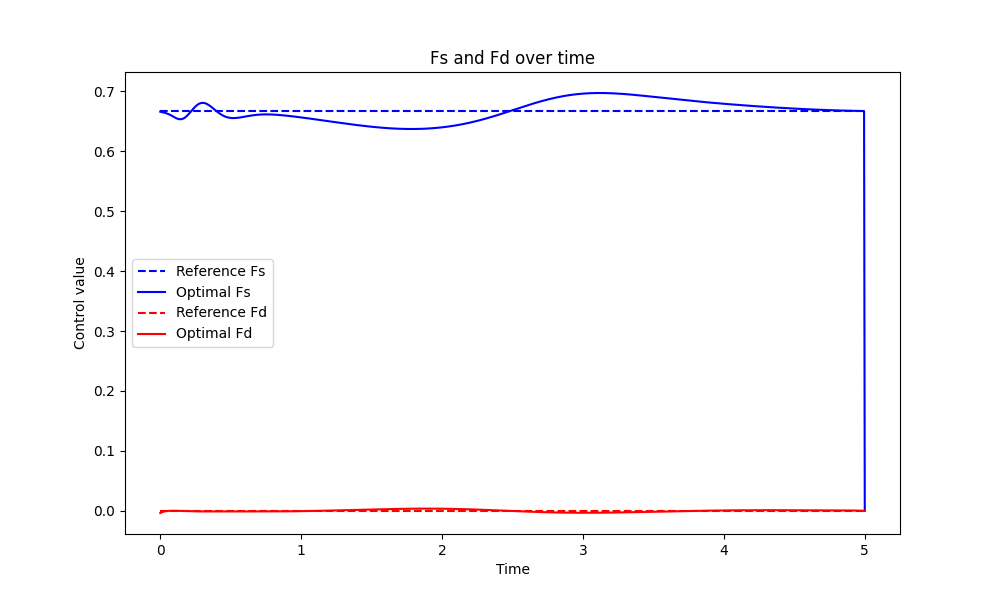
\includegraphics[width=0.85\textwidth]{pictures/Figure_5_opt_smooth.png}
  \caption{Optimal input over time.}
  \label{fig:Reference trajectory}
\end{figure}


\subsection{Suboptimal trajectories}
To illustrate the iterative evolution of the algorithm, we display only the x and y coordinates of the quadrotor over time and the armijos plot, providing an overview of the overall progression. Refer to the code for more details.
\begin{figure}[H]
  \centering
  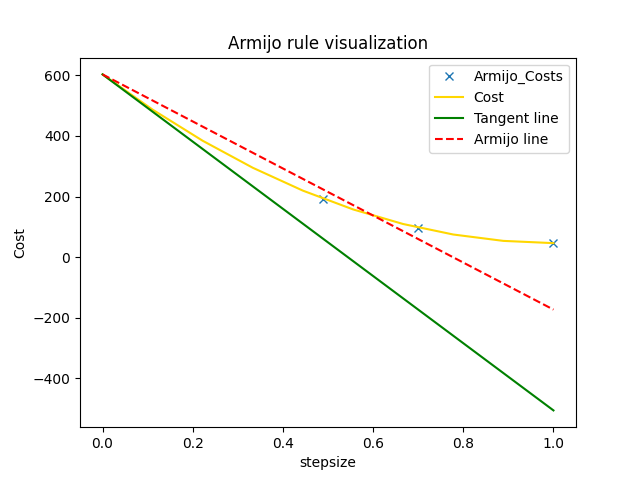
\includegraphics[width=1\textwidth]{pictures/Figure_1_1.png}\hfill \\
  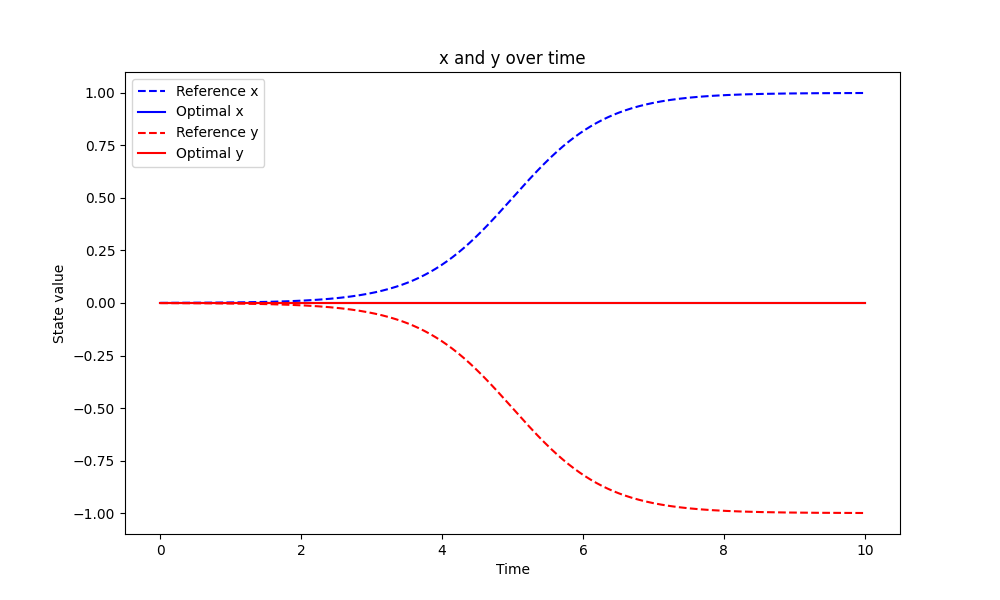
\includegraphics[width=1\textwidth]{pictures/Figure_1_2.png}\hfill
  \caption{First iteration.}
  \label{fig:Reference trajectory}
\end{figure}

\begin{figure}[H]
  \centering
  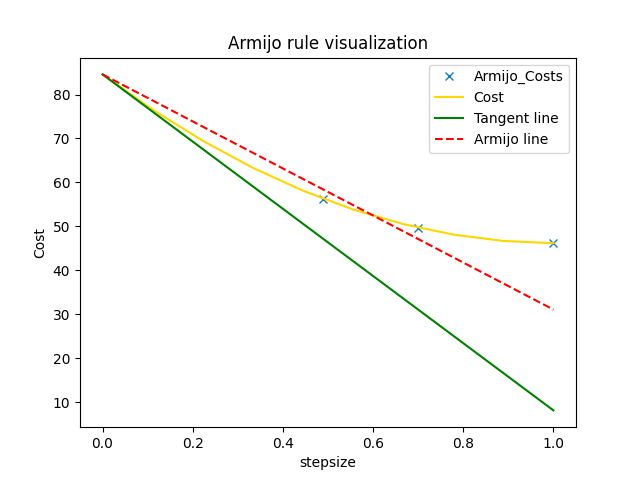
\includegraphics[width=1\textwidth]{pictures/Figure_2_1.png}\hfill \\
  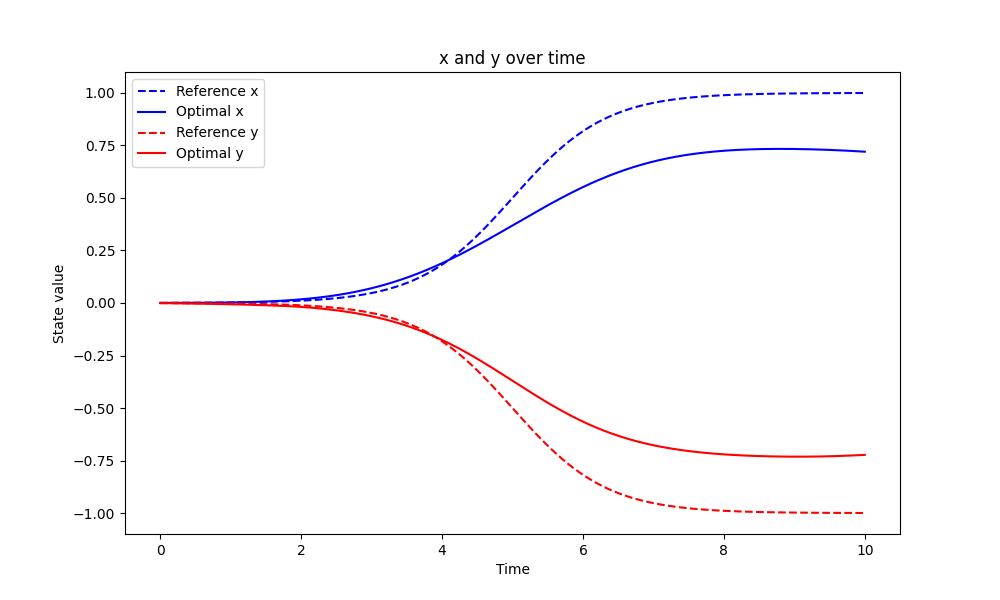
\includegraphics[width=1\textwidth]{pictures/Figure_2_2.png}\hfill
  \caption{Third iteration.}
  \label{fig:Reference trajectory}
\end{figure}

\begin{figure}[H]
  \centering
  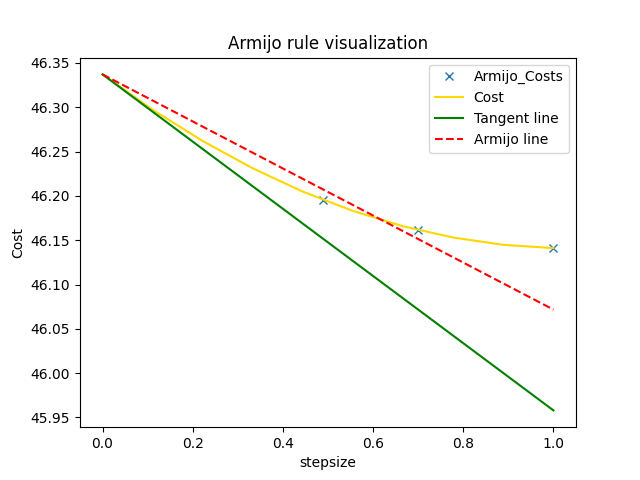
\includegraphics[width=1\textwidth]{pictures/Figure_3_1.png}\hfill\\
  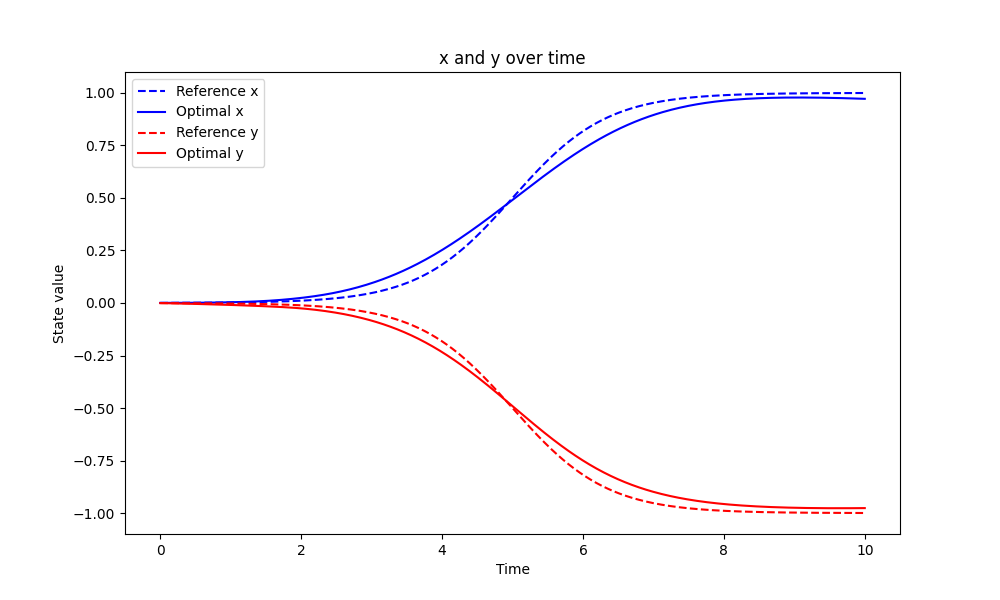
\includegraphics[width=1\textwidth]{pictures/Figure_3_2.png}\hfill
  \caption{Seventh iteration.}
  \label{fig:Reference trajectory}
\end{figure}

\begin{figure}[H]
  \centering
  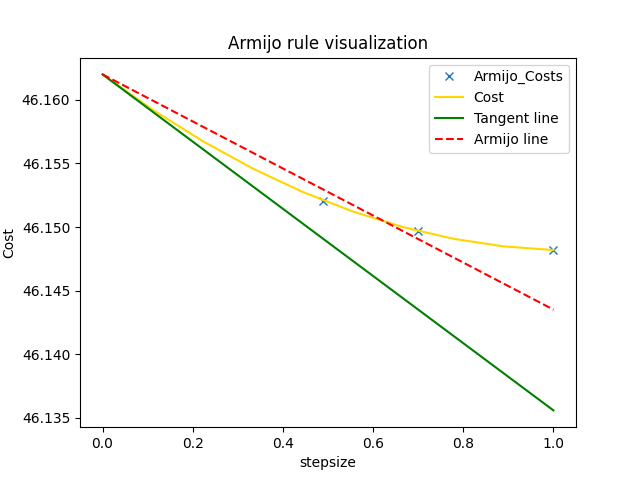
\includegraphics[width=1\textwidth]{pictures/Figure_4_1.png}\hfill\\
  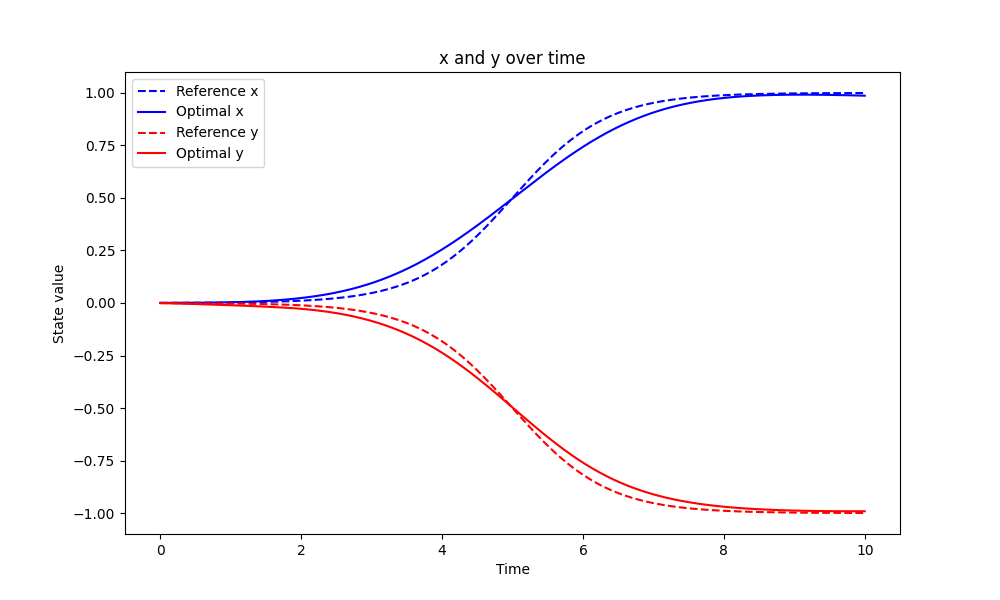
\includegraphics[width=1\textwidth]{pictures/Figure_4_2.png}\hfill
  \caption{Final iteration.}
\end{figure}

On the code you will also find the outcomes of the Linear Quadratic Regulator on the reference trajectory provided by equilibria that are two distinct velocity in space (Case 2).